% Elephant Agent: Personal-Model-First Memory for Personal AI

\documentclass{elephant}

\usepackage[a4paper,margin=2.5cm,headheight=52pt,headsep=18pt]{geometry}
\usepackage{amsmath,amssymb}
\usepackage{enumitem}
\usepackage{tabularx}
\usepackage{longtable}
\usepackage{tikz}
\usepackage[noabbrev,nameinlink]{cleveref}
\usetikzlibrary{arrows.meta,positioning,shapes.geometric,fit,backgrounds,calc}

\hypersetup{
  pdfauthor={Elephant Agent / Agentic Intelligence Lab},
  pdftitle={Elephant Agent: Personal-Model-First Memory for Personal AI}
}

\newcommand{\sysname}{Elephant Agent}
\newcommand{\personalai}{personal AI}
\newcommand{\layermodel}{\textit{System Layer Model}}
\newcommand{\responseLoop}{\textit{Response Loop}}
\newcommand{\reflectionSystem}{\textit{Reflection System}}

\setlength{\emergencystretch}{2em}

\title{Elephant Agent: Personal-Model-First Memory for Personal AI}
\subtitle{Correctable Understanding, Proactive Curiosity, and Local Semantic Recall}

\author{
  Xunzhuo Liu$^{1}$, Hao Wu$^{1}$, Huamin Chen$^{1}$, Xue Liu$^{1,2,3,4}$, Bowei He$^{1,2,3,\dagger}$ \\
  $^1$ Agentic Intelligence Lab, $^2$ MBZUAI, $^3$ McGill University, $^4$ Mila \\
  $^\dagger$ Corresponding author: \texttt{Bowei.He@mbzuai.ac.ae}
}
\date{April 2026}
\abstract{Many personal-agent systems now include memory, and many self-evolving agent
systems treat reusable skill acquisition as the primary path to improvement.
For personal AI, both are downstream of a more central problem: how to maintain
correctable understanding of one person over time. Elephant Agent is a
\emph{personal-model-first} memory architecture for personal AI. It centers a
Personal Model: a durable, grounded understanding across four lenses --- who
the user is (\textit{Identity}), what surrounds them (\textit{World}), what is
alive right now (\textit{Pulse}), and what their path has taught them
(\textit{Journey}).

The system treats memory as five cooperating layers rather than a transcript
archive or a vector store: Matriarch Core / Personal Model, Elephant State,
Episode / Loop / Step Trail, Contextual Recall, and Background Learning. Raw
Steps preserve what happened; contextual recall retrieves support from Steps
and Facts; proactive questions expose gaps, conflicts, stale Pulse, and useful
adaptations; background learning decides when evidence should change durable
claims. There is no free-form memory-note table or foreground memory write
surface. Durable understanding is written through governed Personal Model
tools and remains inspectable, correctable, and source-provenanced.

This report describes the Elephant Agent architecture, four-lens Personal Model
schema, proactive curiosity loop, local semantic recall path, background reflect
pipeline, dashboard inspection surfaces, and evaluation scenarios for wake
recovery, correction, no-match recall, and memory quality over time.
}

\begin{document}

\maketitle

\section{Introduction}
\label{sec:introduction}

Elephant Agent starts from the animal before the architecture. Elephant memory
is not merely large storage. Elephants recognize herd members, remember danger
cues, return to important locations after long gaps, and preserve bonds with
other animals and humans over years. Their hippocampus links emotion to
long-term memory, while their cerebral cortex supports problem solving,
cooperation, tool use, and simple quantitative tracking. In older matriarchs,
memory can become practical judgment for the herd: a remembered drought, route,
or warning sign changes future behavior.

Personal AI has an analogous design problem. It is not only an assistant that
can answer the current prompt. It is an individual system that should become
better at working with a particular person across days, surfaces,
interruptions, corrections, and repeated work. The central improvement target
is therefore not a larger chat window, a longer log, a vector memory store, or
a growing catalog of reusable skills. The central target is the Personal Model:
the explicit object that says what the agent currently understands about the
person, why it believes that, what is uncertain, and what should be asked next.

This distinction matters because many personal-agent systems now include
memory, and many self-evolving agent systems define progress primarily as
acquiring reusable skills, tools, or automations. Those capabilities are
valuable, but they answer different questions. Raw recall asks what can be
retrieved from the past. Skills ask what the agent can do. Personal AI also
needs to answer what it currently understands about the person and how that
understanding should change. Elephant Agent places this third object at the
center. Memory is not discarded or narrowed to retrieval; retrieval becomes one
layer in an architecture that turns episodes, relationships, risk patterns, and
background reflection into correctable understanding. Capabilities can then be
selected as operator-managed tools, but durable personalization remains in
correctable facts, open questions, and source provenance rather than hidden
skill weights or nearest-neighbor notes.

Elephant Agent implements this Personal-Model-first approach as a personal AI runtime
with durable continuity. It records atomic events as Steps, binds them to
execution Loops, groups Loops into Episodes, keeps Elephant State deliberately small,
and evolves the Personal Model through foreground updates, proactive questions,
and background reflect jobs. The clean product-facing memory architecture has
five layers:

\begin{center}
\texttt{Personal Model -> Elephant State -> Step Trail -> Contextual Recall -> Background Learning}
\end{center}

\begin{figure}[t]
  \centering
  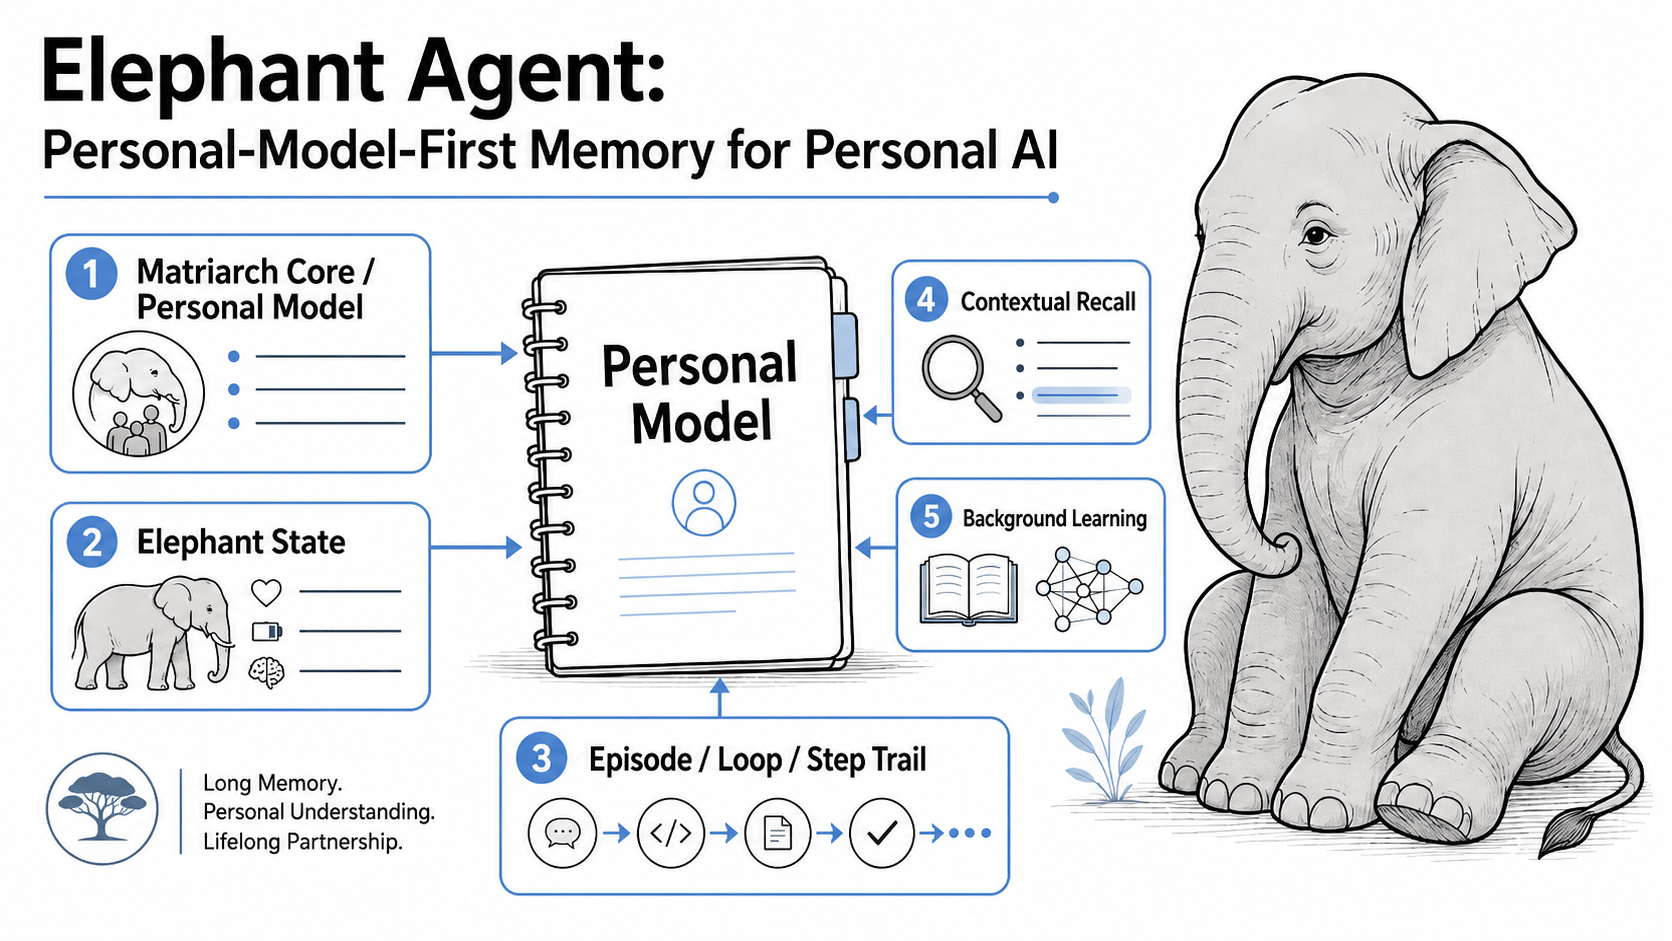
\includegraphics[width=\linewidth]{../../apps/site/static/assets/resources/paper-1.png}
  \caption{Elephant Agent centers personal AI evolution on a correctable
  Personal Model rather than on transcript accumulation or skill growth alone.}
  \label{fig:personal-model-overview}
\end{figure}

The Personal Model is the durable understanding layer. Elephant State carries the
Elephant Agent identity and one natural-language current context note. An Episode is one
wake or open runtime window. A Loop is one model interaction round. A Step is
one atomic event inside a Loop. Together they form the Episode / Loop / Step
trail. Contextual Recall retrieves support from Steps and Facts for the current
turn or a reflect job. Background Learning decides when evidence should change
claims or questions. Steps are the evidence; facts carry their own source
Episode provenance.

This report describes Elephant Agent as a system, not as an implementation plan. The
runtime provides six practical capabilities:

\begin{enumerate}[leftmargin=*]
  \item \textbf{Elephant-based continuity.} Elephant Agent resumes from a durable elephant rather
  than treating a session, thread, or transcript as the owner of continuity.

  \item \textbf{Personal Model evolution.} Long-term user understanding is
  represented as active four-lens facts with confidence, source episodes,
  correction, and governance.

  \item \textbf{Proactive curiosity.} The system can ask at quiet, balanced, or
  active effort levels when a gap, conflict, stale Pulse, or adaptation would
  materially improve future help.

  \item \textbf{Claim-aware recovery.} Explicit user-directed updates change
  active facts in the foreground, while current-turn search can return strong,
  weak, or no match before Elephant Agent relies on recall.

  \item \textbf{Background learning.} Feature-composable reflect agents run on
  Episode close, manual, diary, dream, initialization, and context-compaction
  triggers, then write through the same Personal Model and question tools.

  \item \textbf{Capability use around understanding.} Skills, tools, models,
  cron jobs, messaging adapters, TUI, and Dashboard remain visible capabilities
  around the Personal Model.
\end{enumerate}

The design goal is a personal AI that can answer four operational questions at
any time: what happened, where should this line of work resume, what stable
understanding exists about the user, and whether the Personal Model actually
supports the claim being used now. Elephant Agent answers those questions by making
persistence, provenance, and no-match recovery runtime contracts rather than
prompt tricks.

The rest of the report is organized as follows. \Cref{sec:abstraction}
defines Personal-Model-first evolution and downstream capabilities.
\Cref{sec:architecture} describes the Elephant Agent runtime architecture.
\Cref{sec:continuity-grammar} defines persistence ownership.
\Cref{sec:curiosity} specifies facts and proactive questions.
\Cref{sec:understanding-recovery} covers recall and background learning.
\Cref{sec:implementation-direction} summarizes implementation and evaluation
surfaces. \Cref{sec:related-systems} gives comparison axes, and
\Cref{sec:future-work} outlines the next research and product directions.

\section{Personal-Model-First Memory}
\label{sec:abstraction}

Elephant Agent treats the Personal Model as the primary object of personal AI
improvement. A reusable skill can make an agent more capable, but it does not
by itself say what Elephant Agent currently understands about a specific user. The
Personal Model supplies that owner.

\subsection{Why Skill-First Evolution Is Incomplete}

Skill-first systems optimize for reusable workflows. They can discover that a
tool chain often succeeds, package the path, and make it easier to invoke
later. This is useful, but it leaves the core personal questions unresolved:

\begin{itemize}[leftmargin=*]
  \item What does Elephant Agent currently understand about this user?
  \item Which source Episodes support that understanding?
  \item How can the user correct, forget, or dispute it?
  \item Which question would materially improve future help?
\end{itemize}

These are not skill-package questions. They are Understanding System questions.
Elephant Agent therefore treats skills as ordinary capabilities, while durable
personalization lives in facts, questions, and provenance.

\subsection{Personal Model Contents}

The Personal Model is made of active facts grouped by four lenses:

\begin{center}
\begin{tabularx}{0.98\linewidth}{@{}lX@{}}
\toprule
\textbf{Lens} & \textbf{Purpose} \\
\midrule
Identity & Durable attributes: name, values, decision style, boundaries, and stable self-descriptions. \\
World & The user's environment: people, relationships, projects, tools, domains, places, and stable context. \\
Pulse & Current state: active work, current pressure, recent constraints, priorities, and mood patterns. \\
Journey & Accumulated experience: lessons, failures, recovery patterns, past decisions, and long-running growth. \\
\bottomrule
\end{tabularx}
\end{center}

Every fact has a lens, topic, text, status, confidence, source, and
\texttt{source\_episode\_ids}. Only active facts enter the stable prompt.
Retired and disputed facts remain available for audit but must not shape
answers.

\subsection{Remember Less, Understand Deeper}

The Personal Model is not a complete profile. It is a compact set of claims that
matter for future help. The system should preserve information when it changes
future collaboration, recall, risk judgment, or continuity. It should not
convert every chat detail into durable truth.

This gives the product rule a technical form: remember less, understand deeper.
The durable unit is not a transcript sentence. The durable unit is a correctable
fact with source Episode provenance and an explicit lens/topic.

\subsection{Capabilities as Downstream Tools}

Skills remain useful as operator-controlled procedures. They can be installed,
viewed, enabled, disabled, and invoked when relevant. They are not the owner of
personal truth and are not ranked by a separate hidden affinity model.

The result is a simpler inversion: Elephant Agent does not ask only what the agent can
learn to do. It asks what it currently understands about the person, why that
understanding exists, and how the user can correct it.

\section{Elephant Agent Runtime Architecture}
\label{sec:architecture}

The Elephant Agent runtime is organized around five cooperating memory layers:
Matriarch Core / Personal Model, Elephant State, Episode / Loop / Step Trail,
Contextual Recall, and Background Learning. Foreground response, explicit
Personal Model updates, background reflect, and operator-managed capabilities
all write through governed boundaries, and each durable update remains
traceable to runtime Steps and source Episodes.

\begin{figure}[t]
  \centering
  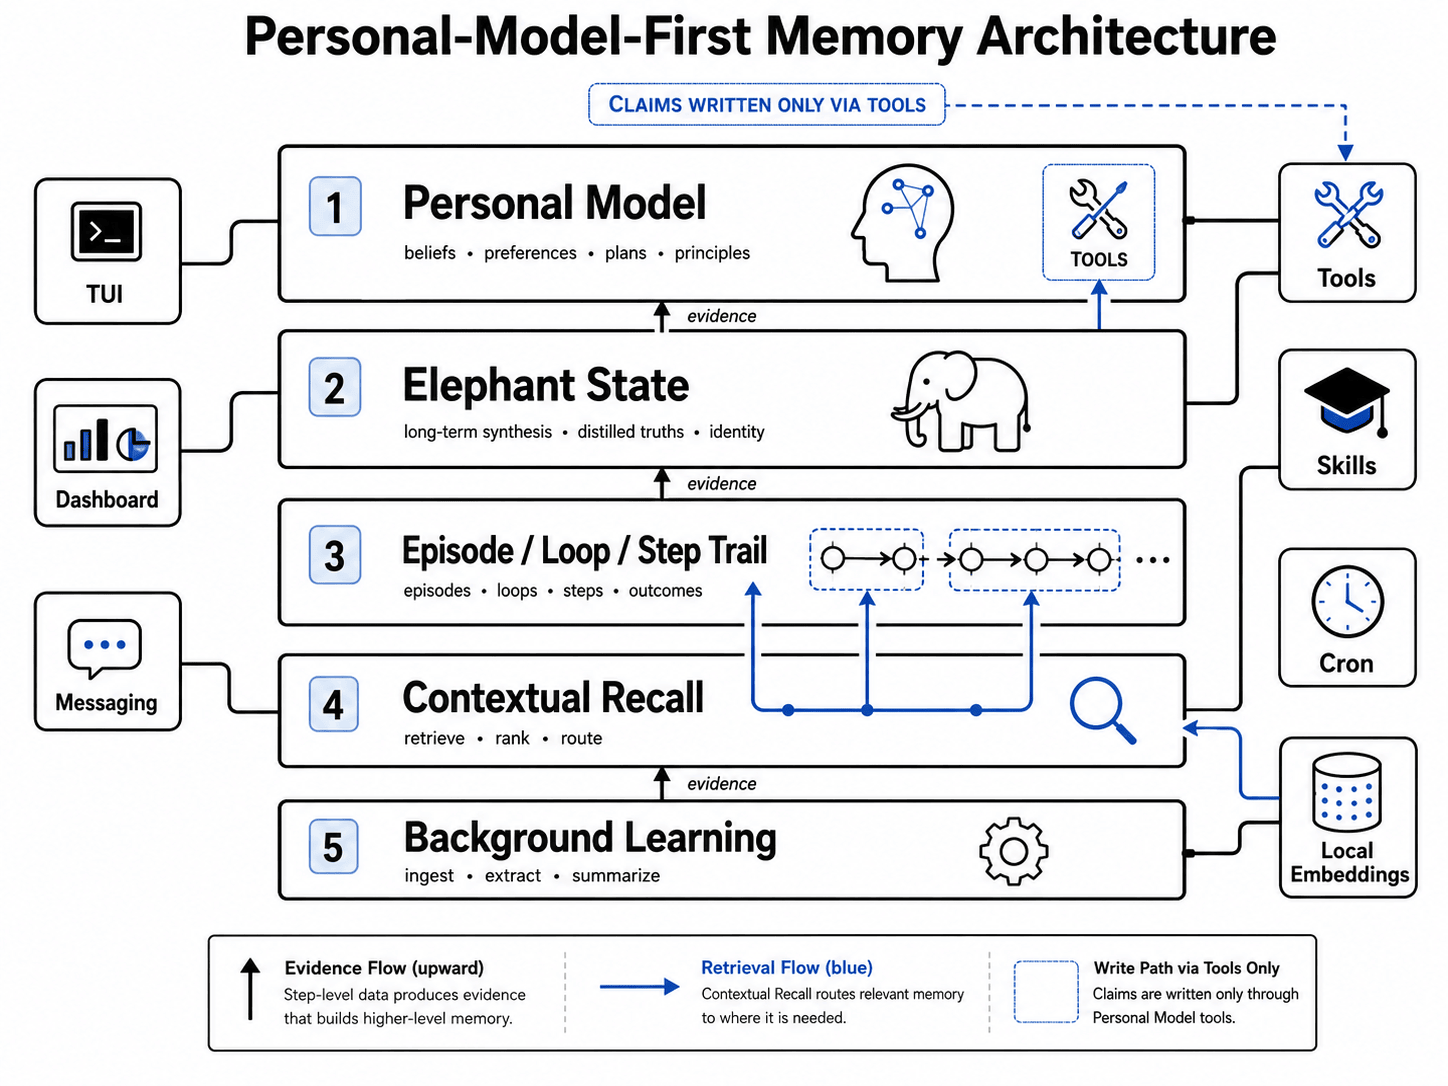
\includegraphics[width=\linewidth]{../../apps/site/static/assets/resources/paper-2.png}
  \caption{Elephant Agent's Personal-Model-first memory architecture. Evidence
  flows upward from Step-level source material; contextual recall retrieves
  support for the current turn; durable claims are written only through governed
  Personal Model tools.}
  \label{fig:runtime-architecture}
\end{figure}

\subsection{Runtime Planes}

The system is easier to reason about as five planes that cooperate at runtime.
The \textbf{surface plane} accepts triggers from the chat TUI, Dashboard,
messaging gateways, API calls, cron jobs, and background jobs. The
\textbf{response plane} owns the current foreground answer: it resolves the elephant,
selects provider and model posture, calls tools, and returns a response,
pause, or handoff. The \textbf{continuity plane} owns Elephant State, Episodes,
Loops, and Steps, so every answer has an execution trail. The
\textbf{understanding plane} owns Personal Model facts and open questions. The
\textbf{learning plane} owns background LearningJobs that read Step packets and
write back through Personal Model tools.

The important design decision is that these planes do not collapse into one
prompt. A wake prompt is a projection of state. It can include the elephant identity,
active facts, a compact Episode opening note, tool policy, and current-turn
recall support. The durable owners remain the tables and tools behind those
projections.

\subsection{Persistence Ownership}

The clean persistence model is organized around ownership boundaries, not a
single memory table:

\begin{center}
\begin{tabularx}{0.98\linewidth}{@{}lX@{}}
\toprule
\textbf{Table} & \textbf{Role} \\
\midrule
PersonalModel & One durable understanding container per user. \\
Facts & Active, retired, or disputed lens/topic claims. \\
OpenQuestions & Proactive curiosity prompts and their lifecycle. \\
State & Elephant identity plus one current context note. \\
Episode / Loop / Step & Runtime windows, interaction rounds, and atomic events. \\
SemanticIndexEntry & Vectorized Step or Fact chunks for contextual recall. \\
LearningJob & Background reflect task queue and result JSON. \\
\bottomrule
\end{tabularx}
\end{center}

Steps are the canonical conversation record. Facts carry source Episode
provenance.

\subsection{Foreground Response}

The foreground response loop is responsible for the current answer or
execution. It resolves the elephant, loads active Personal Model facts and relevant
State context, opens or reuses an Episode, starts a Loop, appends Steps, calls
tools, and produces a response or handoff.

Prompt text is a projection of governed runtime state. It may contain active
facts, an Episode opening resume snapshot, tool policy, and current-turn
\texttt{Current-turn recall support:} support. It is not the owner of those facts.

\subsection{Explicit Personal Model Update}

When the user explicitly asks Elephant Agent to remember, correct, forget, or dispute
something, the runtime treats that statement as foreground intent. The response
Loop calls \texttt{tool.personal\_model.update}. The update request names one
lens and topic, the proposed fact text when applicable, and the reason.

Low-risk, clear, user-directed captures may commit immediately. Ambiguous,
sensitive, identity-changing, cross-person, or high-impact captures require
stronger policy handling. Explicit Personal Model update is allowed in the
foreground because the user asked for it, but it still passes through typed
policy and can retire or dispute older facts.

\subsection{Claim-Aware Retrieval}

Current-turn recovery searches active facts. The search surface supports strict
exact lookup, conceptual semantic lookup, and verification. Exact mode disables
semantic drift and accepts only strict topic, phrase, token, or high-overlap
matches. Verify mode uses stricter
thresholds so weak similarity is not treated as belief. Semantic mode can use
translated or paraphrased query variants supplied by the model.

Every result is a claim-level answer with a status: strong match, weak match,
or no match. This status is part of the runtime contract. No match is a valid
answer when Elephant Agent lacks reliable Personal Model support.

\subsection{Background Reflect}

Inferred learning is handled outside the immediate reply. Background reflect is
a feature-composable agent system. A trigger selects features, the runner
builds an evidence packet from Episode Steps, the sub-agent uses foreground
tools such as \texttt{personal\_model.update} and
\texttt{personal\_model.questions}, and the runner persists its summary in
\texttt{learning\_jobs.result\_json}.

\begin{center}
\texttt{Trigger -> features -> Step packet -> reflect agent -> tools -> result\_json}
\end{center}

Supported trigger families include \texttt{episode\_close}, \texttt{manual},
\texttt{diary}, \texttt{dream}, \texttt{init\_profile}, and
\texttt{context\_compaction}. Reflect is part of Background Learning, not a
separate durable truth layer. It is a lifecycle that writes through existing
tools.

\subsection{Capability Path}

Tools, skills, models, cron jobs, messaging adapters, the chat TUI, and the
Dashboard make Elephant Agent operationally useful. They remain visible capabilities
around the Personal Model. When a workflow should become reusable, it remains
an explicit skill package or operator action. When the user corrects Elephant Agent, the
correction updates a Personal Model fact, not a hidden skill-affinity score.

\section{Runtime Layers and Continuity}
\label{sec:continuity-grammar}

The Elephant Agent layer model defines what persists, for how long, and under which
owner. The layers are ordered from durable understanding to atomic runtime
source material.

\begin{figure}[!t]
  \centering
  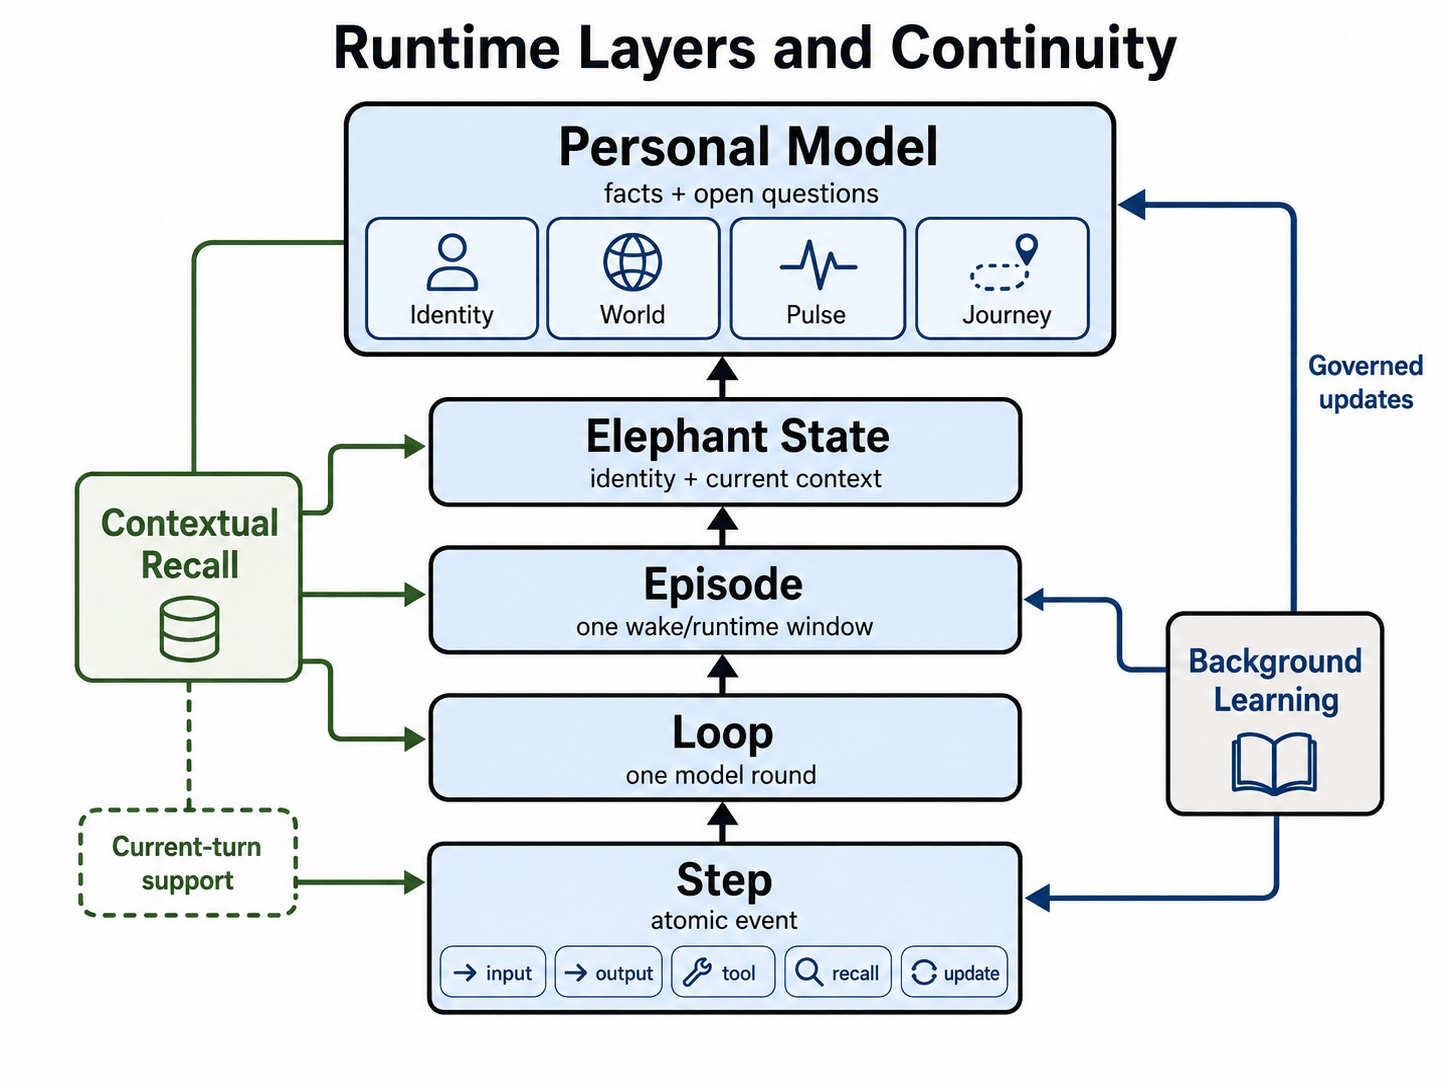
\includegraphics[width=0.86\linewidth]{../../apps/site/static/assets/resources/paper-6.png}
  \caption{The Elephant Agent system layer model, shown from atomic runtime material
  toward durable personalized understanding.}
  \label{fig:layer-model}
\end{figure}

\subsection{Step}

A Step is one atomic event inside a Loop. Examples include user input, model
response, tool call, tool result, recall, Personal Model update, or effective
user query. Steps are not durable memory owners. They are the finest-grained
source material for audit, replay, recovery, debugging, and later reflection.

This distinction prevents impressionistic personalization. Elephant Agent should not
learn directly from an opaque memory sentence. It should learn from structured
events whose source, order, outcome, and artifacts can be inspected.

\subsection{Loop}

A Loop is one model interaction round. It begins with a trigger and ends when
the model response, tool path, or handoff for that round is complete. A short
chat reply is a Loop. A long repair path with many tools may include multiple
Loops.

\subsection{Episode}

An Episode is one open runtime window: a wake, CLI shell window, gateway
worker, API handling window, or background runtime window. Ending an Episode
does not end continuity. A later wake opens a new Episode and resumes from the
same elephant State and Personal Model.

\subsection{Elephant State}

Elephant State is intentionally small:

\begin{center}
\texttt{elephant\_id, display\_name, identity\_text, current\_context\_note, updated\_at}
\end{center}

\texttt{current\_context\_note} is the State-level continuation note produced
by background Episode learning and copied into the next Episode's opening
resume snapshot. It is not a per-turn working memory field and must not become
a hidden task board. Live commitments belong in Episode, Step, current-turn
recall, or explicit task tools.

\subsection{Personal Model}

The Personal Model is the durable understanding layer. It is made of active,
retired, and disputed facts grouped by Identity, World, Pulse, and Journey, plus
open questions that may improve future help. It is not the elephant identity itself.
Deleting an elephant State does not imply deleting the Personal Model.

The simplifying rule is strict: only what should survive across multiple
States, Episodes, and surfaces belongs in the Personal Model. Everything else
should stay in Elephant State, Episode, Loop, Step, or current-turn recall.

\subsection{Wake and Resume}

Wake recovery combines Elephant State and Personal Model. Elephant Agent chooses the target
elephant, opens a new Episode, loads the State resume note, projects active Personal
Model facts, and may inject relevant \texttt{Current-turn recall support:} evidence for the
current turn.

The default wake packet should answer four product questions:

\begin{enumerate}[leftmargin=*]
  \item Who is this elephant and user relationship?
  \item Where did this continuity line leave off?
  \item Which active facts matter now?
  \item What evidence, if any, supports the current query?
\end{enumerate}

This packet is not the durable owner of continuity. It is a projection. If it
is wrong, the system should be able to show which facts, source Episodes, and
Steps produced it.

\section{Proactive Curiosity and Questions}
\label{sec:curiosity}

A key claim of this paper is that a personal AI should improve by forming a
small, correctable understanding of the person, not by accumulating free-form
memory notes. Elephant Agent treats memory as a five-layer architecture:
Personal Model, Elephant State, Episode / Loop / Step trail, Contextual Recall,
and Background Learning. Within that architecture, the durable Personal Model
has two objects: \texttt{Fact} and \texttt{Question}.

\begin{figure}[t]
  \centering
  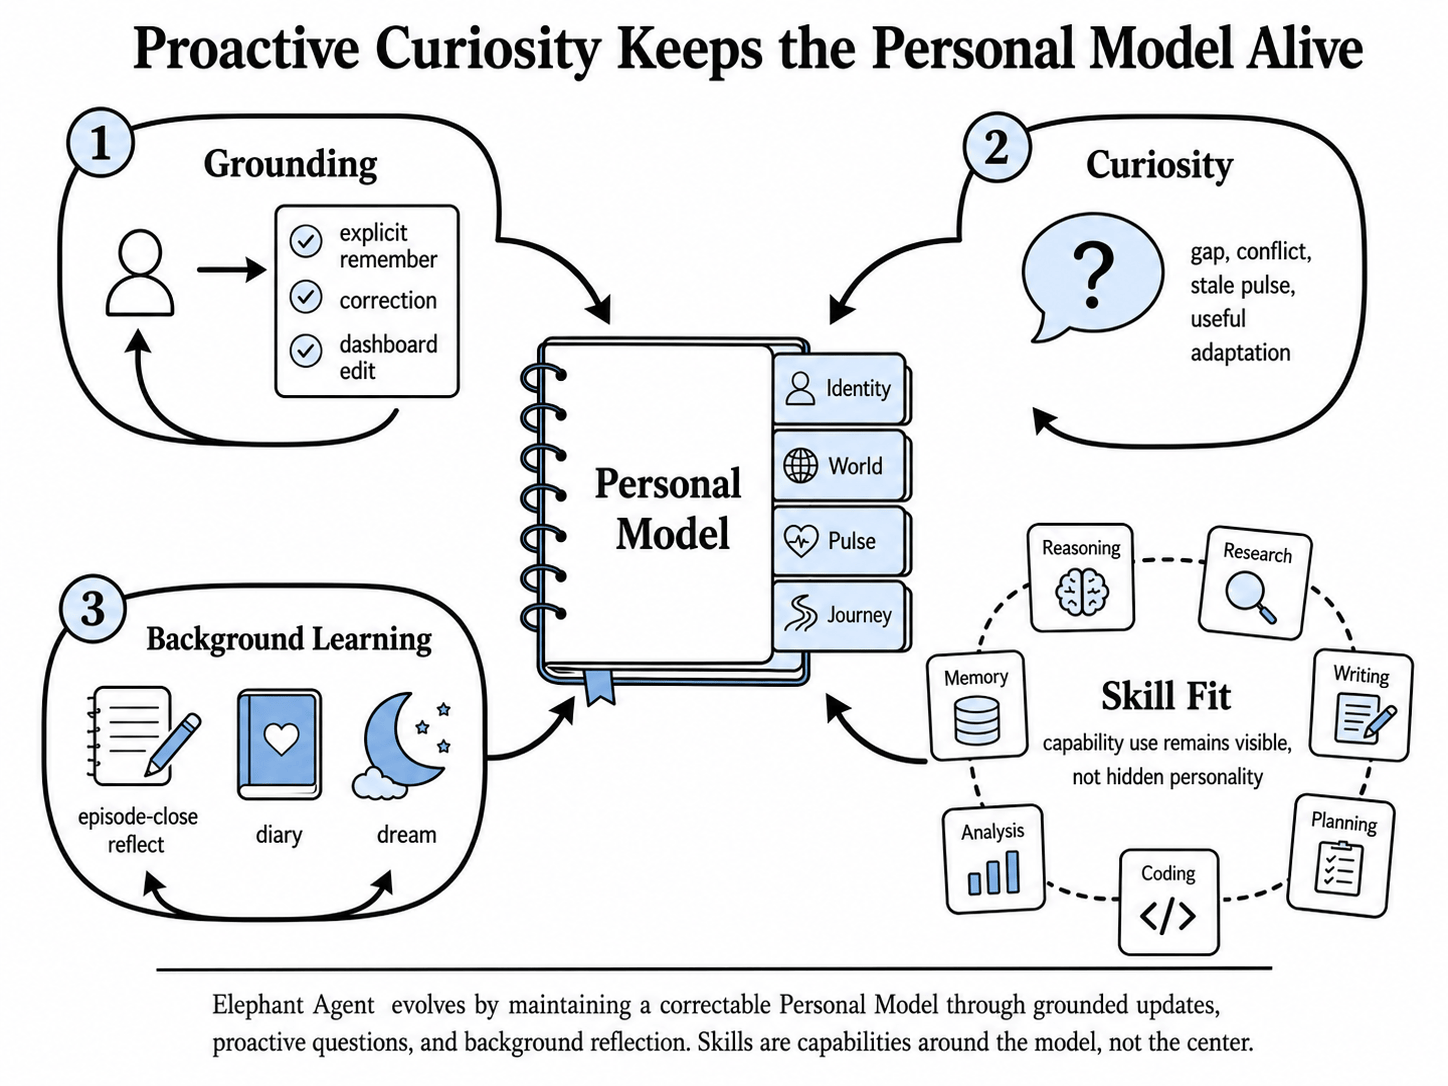
\includegraphics[width=0.9\linewidth]{../../apps/site/static/assets/resources/paper-5.png}
  \caption{Proactive curiosity keeps the Personal Model alive through grounded
  user updates, bounded questions, background learning, and visible skill use
  around the model rather than hidden personality changes.}
  \label{fig:proactive-curiosity-loop}
\end{figure}

\subsection{Facts}

A \texttt{Fact} is the smallest unit of Personal Model truth. Every fact has a
reference, lens, topic, text, status, confidence, source, and
\texttt{source\_episode\_ids}. Statuses are \texttt{active}, \texttt{retired},
and \texttt{disputed}. Only active facts enter the stable prompt.

\begin{description}
  \item[\textit{Identity}] Stable self-description, values, decision style,
  boundaries, and durable preferences.
  \item[\textit{World}] People, relationships, projects, tools, places,
  vocabulary, domains, and stable surrounding context.
  \item[\textit{Pulse}] Current work, current life phase, active pressure,
  recent constraints, priorities, and temporary mood or energy patterns.
  \item[\textit{Journey}] Lessons learned, past experiences, recovery patterns,
  repeated failures, decisions, and long-running growth trajectory.
\end{description}

\subsection{Provenance}

Provenance explains why a fact exists. It is not a separate durable storage
layer. It lives in the entities that reference source material:
\texttt{Fact.source\_episode\_ids}, Step records, and SemanticIndexEntry rows.

When the user asks why Elephant Agent believes something, Elephant Agent traces source Episode
ids, loads relevant Steps, and presents the support material. The support can
help the current turn or inspection flow, but it is not itself prompt truth.

\subsection{Proactive Curiosity and Questions}

A \texttt{Question} is a lens/topic-bound attempt to improve future help. Elephant Agent
creates questions for four reasons only: an important gap, a conflict, a stale
Pulse claim, or a high-value adaptation that would materially change future
behavior. Questions are not a profile-filling checklist.

The product behavior is proactive curiosity rather than a question engine.
Elephant Agent can actively maintain understanding at a user-selected effort level:
\textit{quiet} mostly waits and asks rarely, \textit{balanced} asks at natural
pauses when the answer would help, and \textit{active} is more willing to check
in while still staying optional. These levels govern frequency and willingness
to communicate, not autonomous task execution.

When Elephant Agent asks a question, the lifecycle is explicit: the question moves from
\texttt{open} to \texttt{asked}; the user's answer marks it \texttt{answered};
and the answer is applied through the same Personal Model update path as any
other durable fact. A dismissed question stays visible as a boundary rather
than being re-asked silently. Silence is honored at every effort level.

\subsection{Foreground Tools}

The model-facing surface is deliberately small:

\begin{itemize}
  \item \texttt{tool.personal\_model.search} reads active facts and optional
  provenance.
  \item \texttt{tool.personal\_model.update} is the only foreground write path
  for durable understanding. It supports \texttt{remember}, \texttt{correct},
  \texttt{forget}, and \texttt{dispute}.
  \item \texttt{tool.personal\_model.questions} manages question list, ask,
  answer, and dismiss actions.
\end{itemize}

There is no \texttt{tool.memory.note} in the clean design. Memory is not a
free-form foreground write surface. Current-turn recall is the retrieval layer;
durable understanding changes only through Personal Model tools.

\subsection{Prompt Projection}

Stable prompt projection contains only Elephant identity, active four-lens facts,
the Episode opening resume snapshot when available, and tool policy.
Current-turn retrieval is injected separately as \texttt{Current-turn recall support:}; it is
support for the current turn, not a source of durable truth. Retired facts,
disputed facts, raw memory entries, semantic index rows, and style summaries
are not projected as stable understanding.

\subsection{User Visibility}

The dashboard You page shows the four lenses directly. Each fact can be
corrected, forgotten, or inspected through a \textit{Why} expansion. The
Questions page shows open, asked, answered, and dismissed Personal Model
questions and links answered questions to the facts they produced. This makes
learning inspectable: Elephant Agent does not silently model the user; it maintains a
small set of facts the user can challenge.

\section{Understanding Recovery and Background Learning}
\label{sec:understanding-recovery}

Continuity depends on memory, but memory is not a single retrieval primitive.
Elephant Agent implements memory through five owned layers. Steps capture what
happened. Elephant State keeps one continuity line coherent. The Personal Model
keeps durable cross-line understanding. Contextual Recall retrieves support
from Steps and Facts. Background reflect decides when Step evidence should
support heavier updates.

\subsection{Conversation Search}

\texttt{tool.conversation.search} retrieves past conversation content for the
model. It answers a different question than Personal Model search: where did
this happen in the lived trail? The surface supports two modes. In
\texttt{mode=discover}, it groups matching material into copyable time ranges.
In \texttt{mode=recall}, it returns Step-level evidence from the selected
range. It reads from:

\begin{enumerate}[leftmargin=*]
  \item \textbf{SemanticIndexEntry} for vector similarity over indexed Step or
  Fact chunks;
  \item \textbf{Steps} for time-range fallback when semantic search is cold or
  empty;
  \item \textbf{Episodes} for metadata aggregation in discovery mode.
\end{enumerate}

Steps are the canonical conversation record. Query planning separates the topic
core from recall operators such as recency, current-state, historical, recap,
and verification intent. The planner handles English and CJK temporal phrases,
then retrieval applies explicit windows such as \texttt{last\_night},
\texttt{yesterday}, \texttt{last:3d}, date expressions, or ISO intervals. The
hybrid path searches each allowed scope through vector, BM25, exact keyword,
token-coverage, and n-gram signals, then reranks with a small intent-aware time
score. Semantic relevance remains primary; recency only breaks near ties or
helps when the user explicitly asks for recent material.

\subsection{Claim-Aware Personal Model Search}

When Elephant Agent needs long-term user context, it does not retrieve a generic profile
blob or nearest-neighbor memory chunk. It searches active Personal Model facts.
The retrieval unit is the fact, and source Steps remain support for the current
turn rather than truth by themselves.

\begin{figure}[t]
  \centering
  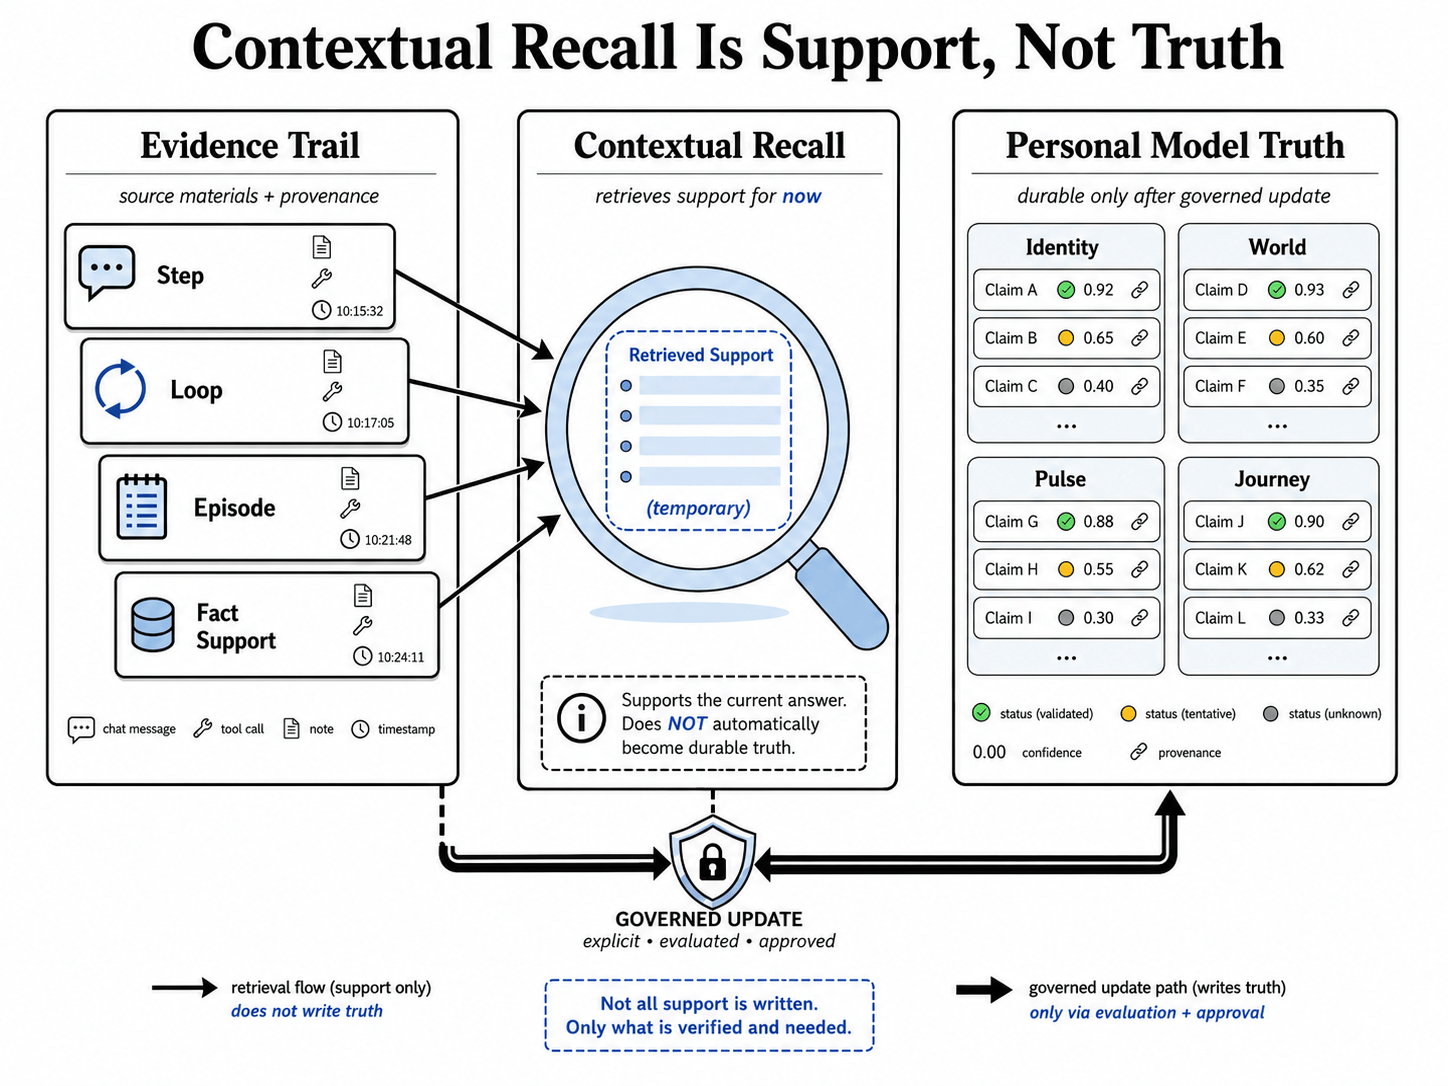
\includegraphics[width=0.9\linewidth]{../../apps/site/static/assets/resources/paper-4.png}
  \caption{Contextual Recall retrieves temporary support from the evidence
  trail, while durable Personal Model truth changes only through governed
  update paths with status, confidence, and provenance.}
  \label{fig:contextual-recall-support}
\end{figure}

The foreground search surface combines several deterministic and semantic
signals:

\begin{itemize}[leftmargin=*]
  \item topic, fact text, and source-support matches;
  \item Unicode lexical matching and CJK n-gram overlap;
  \item weak fuzzy matching for small spelling or character variation;
  \item semantic candidates from the durable index;
  \item optional translated or paraphrased query variants supplied by the model;
  \item lightweight polarity agreement or conflict for clear preference statements.
\end{itemize}

The result is thresholded. A search can return \texttt{strong\_match},
\texttt{weak\_match}, or \texttt{no\_match}. This is an important safety
property: if Elephant Agent cannot find a reliable active fact, it should expose the gap
rather than fabricate Personal Model support.

\subsection{Multilingual Hybrid Time-Aware Search}

The two search surfaces share a common retrieval posture but preserve different
truth semantics. Conversation search retrieves evidence from Steps and Episode
summaries. Personal Model search retrieves active claims. Both rely on a
multilingual hybrid search strategy:

\begin{figure}[t]
  \centering
  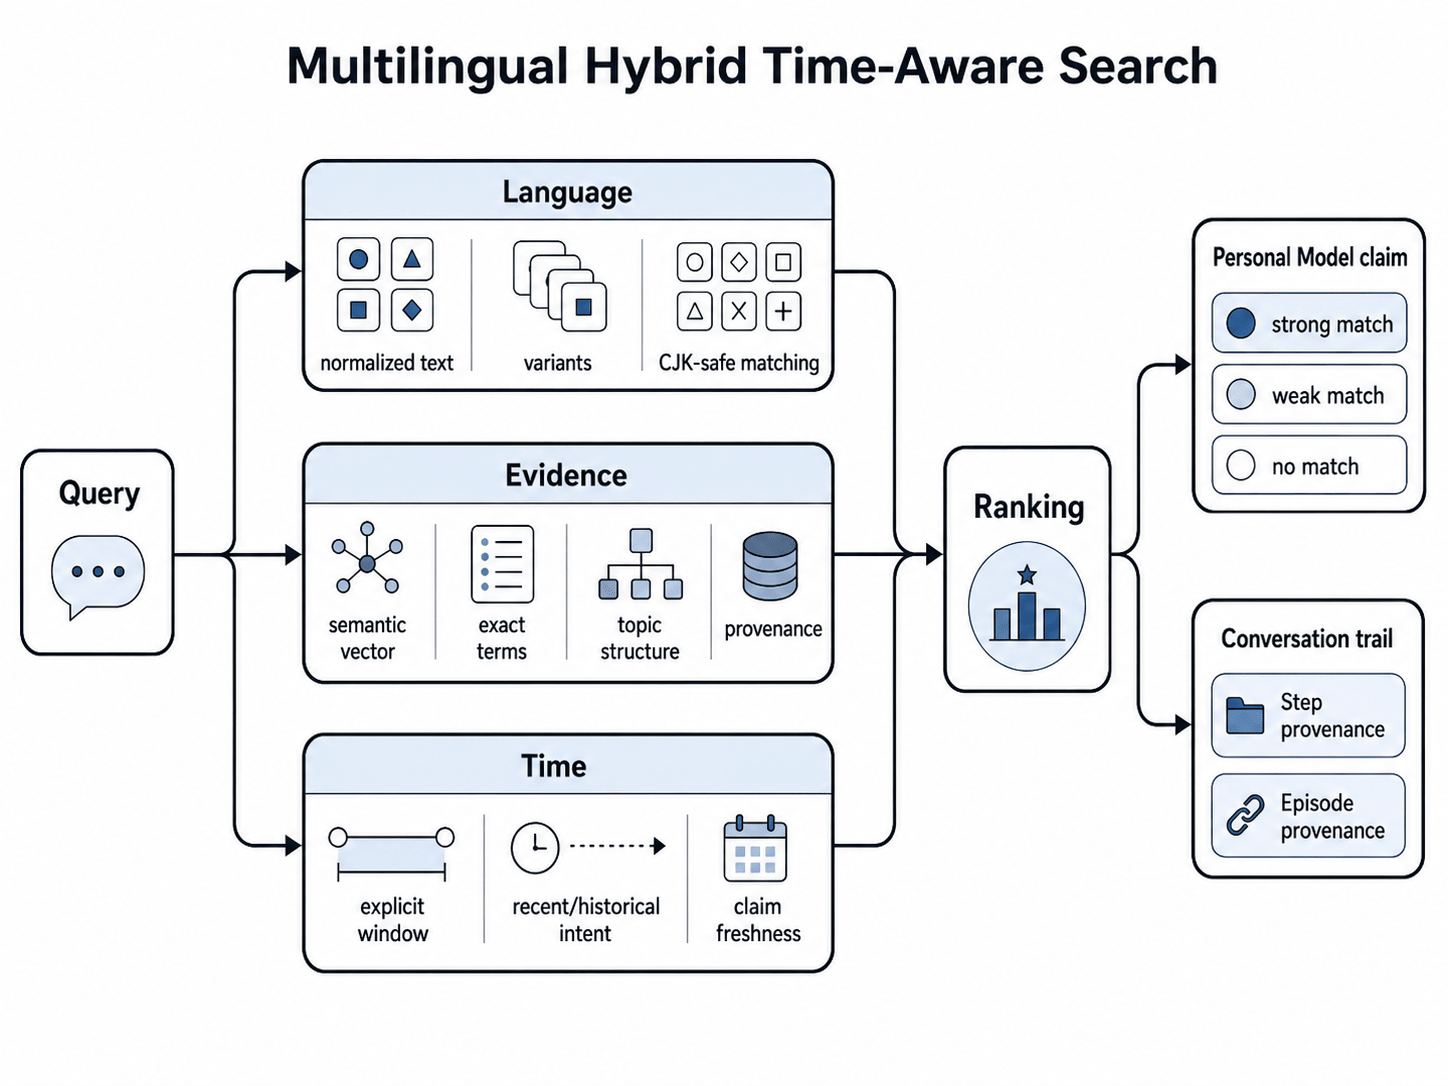
\includegraphics[width=0.9\linewidth]{../../apps/site/static/assets/resources/paper-7.png}
  \caption{Multilingual hybrid time-aware search separates query shaping,
  evidence fusion, and temporal judgment before returning either Personal Model
  claim support or Conversation trail provenance.}
  \label{fig:multilingual-hybrid-time-aware-search}
\end{figure}

\begin{enumerate}[leftmargin=*]
  \item \textbf{Query shaping.} The runtime normalizes Unicode text, preserves
  mixed-language tokens, expands CJK tokens into character n-grams, and accepts
  model-supplied translated or paraphrased \texttt{query\_variants}.
  \item \textbf{Candidate generation.} Hybrid search fuses vector similarity,
  BM25, token coverage, exact keyword matches, and n-gram overlap over the
  scoped semantic index. Personal Model search also adds fielded topic/fact
  matches and source-support text.
  \item \textbf{Time awareness.} Conversation search applies explicit time
  windows and intent-aware recency or historical reranking. Personal Model
  search applies volatility-based freshness so permanent claims remain stable,
  while situational and ephemeral claims lose rank when they have not been used
  recently.
  \item \textbf{Judgment boundary.} Retrieval returns support, not prompt truth.
  Personal Model results are thresholded into \texttt{strong\_match},
  \texttt{weak\_match}, or \texttt{no\_match}; conversation results retain
  Episode, Loop, Step, and source-record provenance.
\end{enumerate}

This lets the system recover a Chinese query over an English thread, or an
English query over a Chinese claim, without relying on a global alias table or
treating nearest-neighbor text as durable understanding.

\subsection{Local Semantic Recall}

Elephant Agent supports a local default embedding path for semantic recall. The local
path lets the user run claim and conversation retrieval without requiring an
external embedding provider. When desired, the embedding provider can be
overridden with a configured remote endpoint and dimensions.

\begin{sloppypar}
The default local provider is \texttt{elephant-local-embed}. It is backed by
\nolinkurl{elephant-embeddings-v1-text-small}, distributed as
\nolinkurl{llm-semantic-router/elephant-embeddings-v1-text-small} on Hugging Face and
\nolinkurl{agentic-intelligence-lab/elephant-embeddings-v1-text-small} on
ModelScope. The runtime loads the model from the local Elephant Agent model root with
\texttt{SentenceTransformer(..., local\_files\_only=True)}.
\end{sloppypar}

The provider exposes three online dimensions: 64, 256, and 768. A lower
dimension gives faster everyday recall; a higher dimension carries more
semantic detail for deeper search. The implementation normalizes vectors and
uses sentence-transformers' truncation path for the selected dimension, so the
same local model can support multiple latency/depth postures.

This is a support-model capability, not the durable truth layer. Embeddings
help find candidate Steps or Facts. The final Personal Model truth remains the
active fact with its status, lens, topic, confidence, and source Episode ids.

\subsection{Background Reflect}

Background reflect is a feature-composable agent system. A trigger fires, a
feature set is resolved, the runner composes a prompt and tools, the sub-agent
receives an evidence packet built from Episode Steps, and the agent calls
tools directly:

\begin{center}
\texttt{episode\_close -> pm/questions/recall -> personal\_model.update}
\end{center}

Feature groups include:

\begin{itemize}[leftmargin=*]
  \item \texttt{pm}: search and write Personal Model facts;
  \item \texttt{questions}: create, settle, or dismiss questions;
  \item \texttt{recall}: search conversation history for support;
  \item \texttt{diary}: write reflective daily entries;
  \item \texttt{skills}: audit visible skill fit without creating hidden
  Personal Model truth;
  \item \texttt{compress}: check compressed content for data loss.
\end{itemize}

Reflect does not use intermediate observations, proposals, or groundings. It
reads Steps directly, writes facts or questions directly through tools, and
persists its run summary in \texttt{learning\_jobs.result\_json}.

\subsection{Deletion, Correction, and Repair}

Durable understanding increases the need for repair. Elephant Agent treats correction as
a normal operation, not an exceptional failure. Corrections can retire active
facts, dispute claims until the user clarifies them, or replace an older fact
for the same lens/topic.

Persistence is valuable only when the user can inspect and correct what
persists. Elephant Agent therefore treats repair paths as part of the runtime contract.

\section{Implementation and Evaluation}
\label{sec:implementation-direction}

Elephant Agent is implemented around the clean Understanding System boundary. The
important implementation property is not that every old object is preserved; it
is that each durable behavior has a single owner and a single correction path.

\subsection{Runtime Records}

The runtime separates Episodes, Loops, and Steps from durable understanding.
Episodes mark open runtime windows. Loops record interaction rounds. Steps
record atomic events for audit and replay. The Personal Model stores active
facts and questions. Elephant State stores the elephant identity plus one natural-language
current context note.

This separation lets the system compact without losing causal structure. A long
tool sequence can be summarized at the Episode level while preserving critical
Step links. A Personal Model fact can be corrected without mutating the
transcript or treating support material as truth.

\subsection{Foreground Update Path}

All foreground durable understanding changes go through
\texttt{tool.personal\_model.update}. The tool writes one lens/topic fact at a
time and supports four actions: remember, correct, forget, and dispute. Init
answers, dashboard corrections, question answers, and chat-time user
corrections all converge on the same path.

\subsection{Claim-Aware Recall and Prompt Projection}

Current-turn retrieval is contextual recall, one layer of the broader memory
architecture. It is injected as \texttt{Current-turn recall support:} when useful
and omitted otherwise. Stable prompt projection contains active
facts only, grouped by Identity, World, Pulse, and Journey, plus the Elephant
identity and Episode opening resume snapshot.

The implementation treats Personal Model search as claim-aware retrieval. The
search tool supports \texttt{topic}, \texttt{query\_variants}, and
\texttt{mode=auto|inventory}. It merges fielded topic/fact/support
matches, Unicode lexical and CJK n-gram signals, weak fuzzy matches, semantic
candidates, and lightweight polarity agreement or conflict. Results are
thresholded into \texttt{strong\_match}, \texttt{weak\_match}, or
\texttt{no\_match}; diagnostics can expose per-fact signals for evaluation but
are not prompt truth.

Topics are represented as facets: stable keys under the four lenses that attach
each claim to one slice of understanding without adding a second profile schema.

\texttt{tool.conversation.search} provides the complementary evidence path. A
small deterministic query planner strips recall operators from the topic core
and detects recency, current-state, historical, recap, and verification intent
across English and CJK phrasing. \texttt{mode=discover} requires a time range
and returns candidate windows; \texttt{mode=recall} retrieves Step or Episode
evidence from a selected window. The searcher first attempts the durable
semantic index with vector, BM25, exact keyword, token-coverage, and n-gram
signals, then falls back to Step scanning when the index is cold. Final ranking
keeps semantic relevance primary and uses temporal intent only as a small
recency or historical tie-breaker.

\subsection{Operational Evaluation}

Elephant Agent is evaluated through longitudinal scenarios rather than single-turn prompt
quality alone:

\begingroup
\small
\setlength{\LTpre}{0.55em}
\setlength{\LTpost}{0.55em}
\begin{longtable}{@{}p{0.22\linewidth}p{0.72\linewidth}@{}}
\toprule
\textbf{Scenario} & \textbf{Expected behavior} \\
\midrule
\endfirsthead
\toprule
\textbf{Scenario} & \textbf{Expected behavior} \\
\midrule
\endhead
Wake recovery & Resume an episode using the Elephant context note, active facts,
and relevant recall. \\
Claim correction & Replace an active fact through \texttt{correct}, retire the
old fact, and project only the new fact next turn. \\
Forget & Retire a fact through \texttt{forget} so it no longer shapes replies. \\
Question answer & Mark the question answered and create the resulting fact
with source Episode provenance. \\
Why inspection & Show source Steps behind a fact without promoting those Steps
to prompt truth. \\
Search no-match & Return no active fact, with a reason, when query quality or
scores are too weak to support an answer. \\
Verify mode & Require stronger support before treating a retrieved fact as
support for a proposed statement. \\
Local recall & Retrieve relevant Step or Fact chunks through the local embedding
path without requiring external embedding services. \\
Multilingual search & Recover relevant claims or Step evidence when the query
and stored material use different languages or mixed-language phrasing. \\
Time-aware search & Respect explicit time windows and temporal intent without
letting recency override stronger semantic or lexical evidence. \\
Local inference posture & Verify that \texttt{elephant-local-embed} can steady,
index, and retrieve at 64, 256, and 768 dimensions with the same Step/Fact
corpus. \\
Background reflect & Run a feature-scoped learning job and persist its summary
in \texttt{learning\_jobs.result\_json}. \\
\bottomrule
\end{longtable}
\endgroup

The evaluation question is whether Elephant Agent can continue the right work with the
right current understanding, and whether the user can correct that
understanding when it is wrong.

\subsection{Case Study Shapes}

The most informative case studies are multi-session and multi-surface:

\begin{itemize}[leftmargin=*]
  \item a repository refactor where Elephant Agent resumes with the correct Elephant context
  and recalls only relevant support;
  \item a design discussion where a correction to collaboration style changes
  the next reply;
  \item a dashboard fact correction where the old fact is retired and the new
  fact appears in the prompt;
  \item an answered Personal Model question that becomes an Identity, World,
  Pulse, or Journey fact with inspectable provenance;
  \item a recall query that correctly returns \texttt{no\_match} instead of
  inventing support;
  \item a background diary or Episode-close job that updates the Personal Model
  through tools and stores a learning result.
\end{itemize}

The reporting unit is the complete lifecycle: trigger, recalled support,
runtime action, fact update, provenance path, dashboard visibility, and later
wake behavior.

\section{Related Systems and Comparison Axes}
\label{sec:related-systems}

This report does not add unverified citations. A citation-verified related
systems pass should be added later through programmatic reference checks rather
than memory-based BibTeX entries. The comparison axes are still clear.

\begin{itemize}[leftmargin=*]
  \item \textbf{Stateless chat systems.} These optimize the current prompt but
  do not preserve durable collaboration state.

  \item \textbf{Long-context systems.} These extend the input window but do not
  by themselves define what should become State or Personal Model truth.

  \item \textbf{Memory-augmented assistants.} These retrieve prior snippets,
  but often leave explicit capture, inferred personalization, maturity,
  correction, and scope boundaries underspecified.

  \item \textbf{Workflow agents.} These execute tool-heavy tasks, but often
  treat persistence as logs and checkpoints rather than as a layered personal
  model.

  \item \textbf{Companion systems.} These move closer to Elephant Agent when they model
  the user, relationship, and elephant identity boundaries, but they often blur
  Episode, State, Personal Model, and procedural learning.

  \item \textbf{Skill and automation systems.} These make repeated workflows
  reusable, but they rarely define the boundary between durable personal
  understanding and executable skill artifacts.

  \item \textbf{Skill-first self-evolving agents.} These optimize for acquiring
  reusable skills, tools, or workflows. Elephant Agent treats that as useful capability
  work, but not as the center of personal AI. The center is the Personal Model:
  active facts, source provenance, and useful questions.
\end{itemize}

Elephant Agent is therefore best compared on ownership boundaries. Atomic events belong
in Steps. Execution belongs in Loops. Wake windows belong in Episodes.
Workline continuity belongs in State. Long-term personalization belongs in the
Personal Model. Background reflect turns Step source material into fact changes
and question candidates without collapsing learned truth into a skill package.

\section{Future Work}
\label{sec:future-work}

Elephant Agent opens five concrete research and product directions.

\begin{figure}[t]
  \centering
  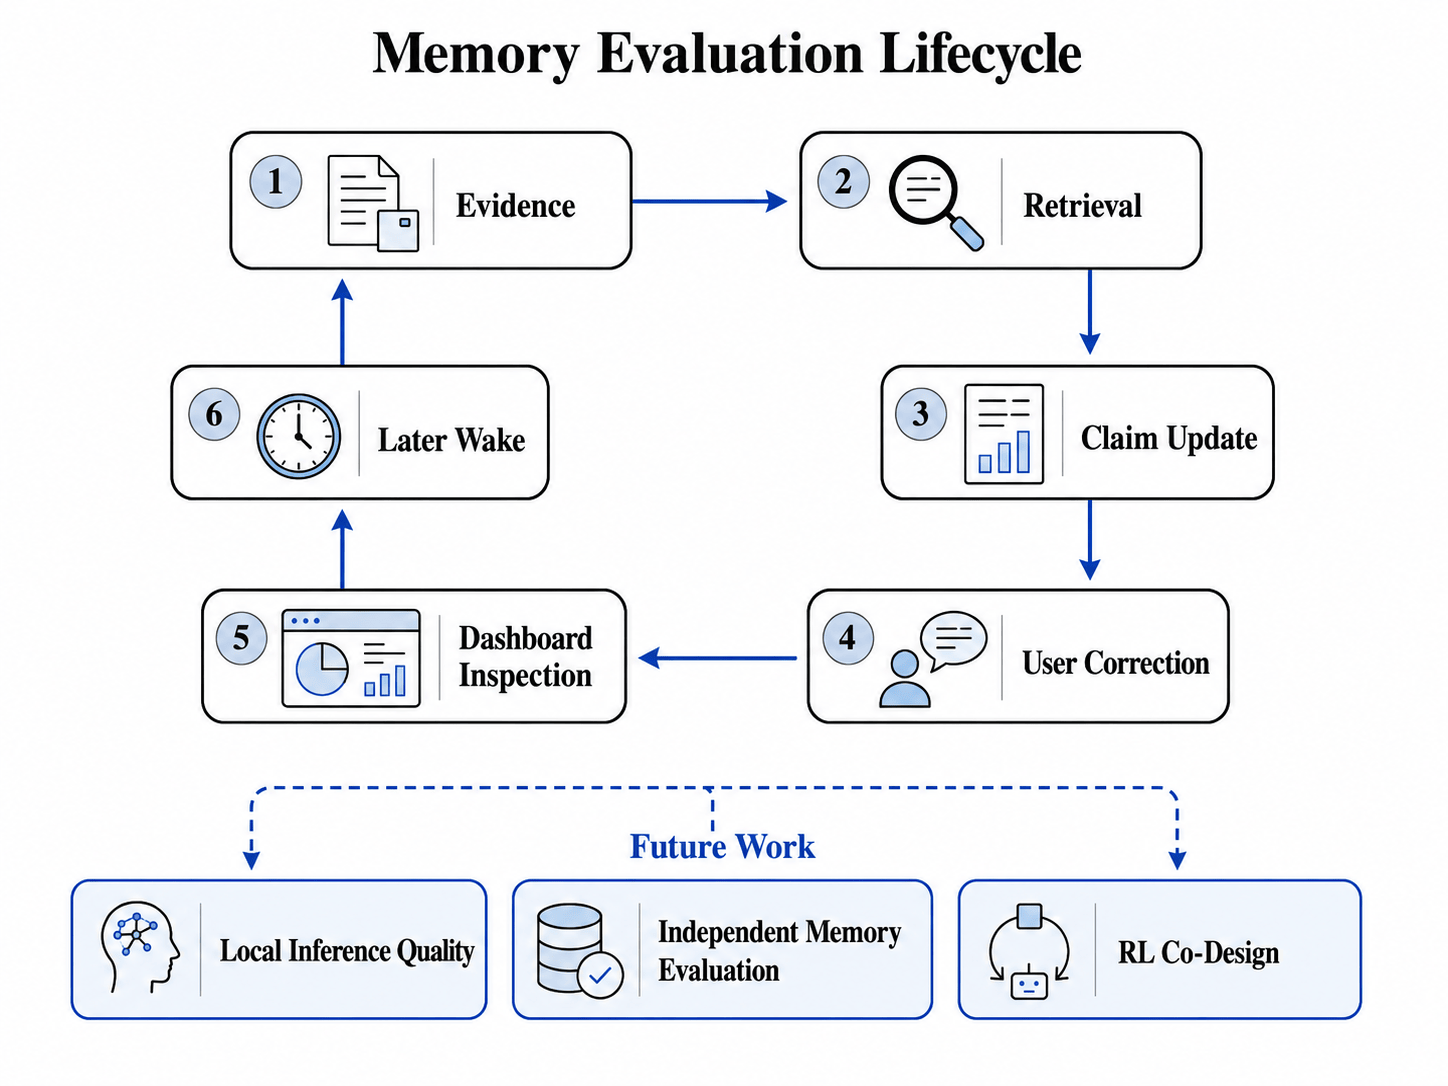
\includegraphics[width=0.9\linewidth]{../../apps/site/static/assets/resources/paper-3.png}
  \caption{Memory evaluation should measure the full lifecycle: evidence,
  retrieval, claim update, user correction, dashboard inspection, and later wake
  behavior, with future work focused on local inference quality, independent
  memory evaluation, and co-design with routing and inference systems.}
  \label{fig:memory-evaluation-lifecycle}
\end{figure}

First, local inference should become faster and more semantically reliable.
The current local path uses a compact sentence-transformers model with
64/256/768 dimensional retrieval modes. Future work should improve latency,
multilingual hybrid recall quality, time-aware ranking calibration,
stance-aware matching, claim-local query expansion, and robustness under
long-running local indexes while keeping active prompt truth in Personal Model
facts.

Second, memory evaluation should become independent of generic chat quality.
Useful benchmarks should measure wake recovery, correction latency, Personal
Model maturity, no-match calibration, social and risk recall, background
learning precision, and whether later answers improve without overriding user
corrections. The evaluation unit should be a lifecycle: evidence, retrieval,
claim update, user correction, dashboard visibility, and later wake behavior.

Third, background skill learning should grow beyond affinity estimation.
Skill affinity is only the first signal: it tells the system which existing
skills fit the user's work and style. A mature background learner should also
notice repeated workflows in the Step trail, propose new user-owned skills when
history reveals a stable pattern, and suggest refinements to existing skills
when evidence shows that a procedure is brittle, stale, or missing local
context. This should remain governed by provenance and operator visibility: the
system may propose or improve skill material, but durable skills should be
inspectable and correctable rather than hidden adaptations.

Fourth, the security boundary should become a first-class research surface.
Personal-model-first agents combine long-lived understanding with tools, code
execution, messaging bridges, and background jobs. Future work should harden
coding sandbox isolation, tool access control, permission scoping, secret
handling, audit trails, and policy checks that decide which tools a foreground
or background agent may call. The important unit is not only a single tool
invocation, but the whole path from recalled support to model decision to tool
execution to durable write.

Fifth, memory should be co-designed with routing, inference, and reinforcement
learning rather than optimized as an isolated retrieval feature. The end-to-end
path is:

\begin{center}
\texttt{agent -> router -> inference -> train}
\end{center}

The routing layer should learn when a turn needs Personal Model search,
conversation search, local embedding, a stronger model, a safer model, or no
recall at all. This naturally connects to vLLM Semantic Router: route by memory
need, language, latency, privacy posture, jailbreak risk, tool-access risk,
confidence, and model-collaboration shape rather than by model cost alone. It
also connects to the vLLM inference engine: local and served inference should
expose latency, batching, cache, and KV-cache optimization signals so Elephant
Agent can choose the right recall and generation posture per turn.

The training side of this co-design is RL post-training over the full agent
lifecycle. The target is not only better tool use or higher task completion.
Training signals should reward asking at the right time, refusing weak memory
support, preserving user corrections, choosing when to write or not write a
claim, selecting the right search surface, using skills only when they fit the
current Personal Model and consent context, and routing through the right model
and inference posture for the user's privacy and safety constraints.

\section{Conclusion}
\label{sec:conclusion}

Elephant Agent implements Personal-Model-first memory for personal AI. The
system does not treat reusable skill acquisition or raw recall as the primary
improvement target. It treats the Personal Model as the center: the durable,
grounded model of the user across Identity, World, Pulse, and Journey.

The clean Understanding System gives that center a concrete path:

\begin{center}
\texttt{Personal Model -> Elephant State -> Step Trail -> Contextual Recall -> Background Learning}
\end{center}

The Personal Model stores active facts and open questions. Elephant State keeps
identity and one current context note. The Episode / Loop / Step trail records
atomic source material. Contextual Recall retrieves support without turning it
into prompt truth. Background Learning reads Steps directly, writes through the
same foreground tools, and persists learning results for inspection.

This structure changes how personal AI improves. Resuming is not transcript
replay, and learning is not only adding reusable skills. Instead, explicit
Personal Model updates are controlled, proactive curiosity operates at the
user's chosen effort level, inferred personalization matures through reflection,
and current-turn recall searches active claims with no-match as a safe outcome.

The practical outcome is a personal AI that can explain what happened, continue
the right line of work, update long-term understanding through governed
provenance, repair itself after correction, and use capabilities while keeping
durable understanding inspectable. Skills still matter. In Elephant Agent, they remain
downstream operator-managed tools around an evolving Personal Model.


% A citation-verified bibliography pass should be added in a later revision.

\end{document}
